\graphicspath{{./ch_theory_and_methods/figures/}}


\chapter{Experimental control and theory of the NV center}
\label{ch:CDL}

\begin{center} 
    \vspace{-1cm} {M.S.~Blok} 
\end{center}


\vspace{-0.5cm} 
NV center has emerged as excellent system to demonstrate quantum control of single spins. While many early demonstrations

\clearpage

\section{Introduction}

\section{The NV center in diamond}
\begin{figure*}
	\centering
	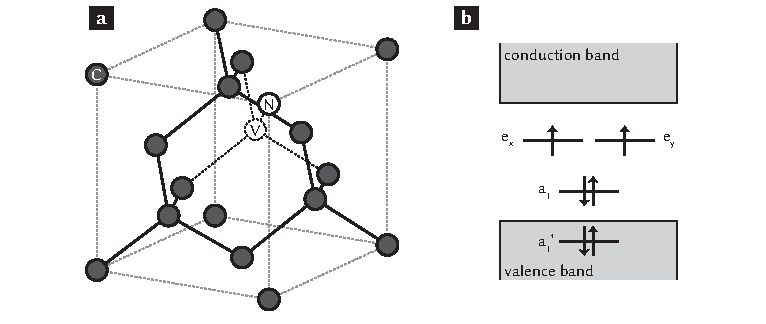
\includegraphics{figure_NV-structure-bernien}
	\caption{\label{fig:tam-fig1-nvstruct} \textbf{} (a) }
\end{figure*}

\begin{figure*}
	\centering
	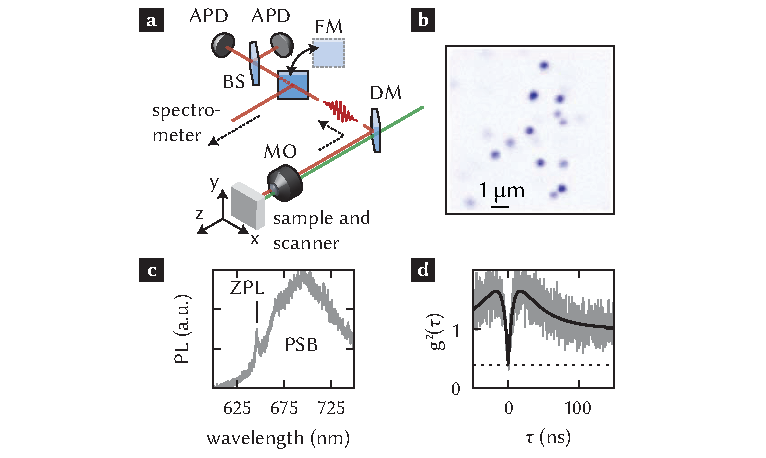
\includegraphics{figure_single_NVs-bernien}
	\caption{\label{fig:tam-fig2-nvstruct} \textbf{} (a) }
\end{figure*}


\section{Single NV center device}
\begin{figure*}
	\centering
	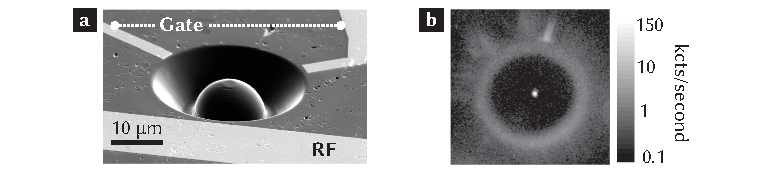
\includegraphics{figure_SIL_finished-bernien}
	\caption{\label{fig:tam-fig3-device} \textbf{} (a) }
\end{figure*}

\section{Addressing the electron excited state with optics}
\begin{figure*}
	\centering
	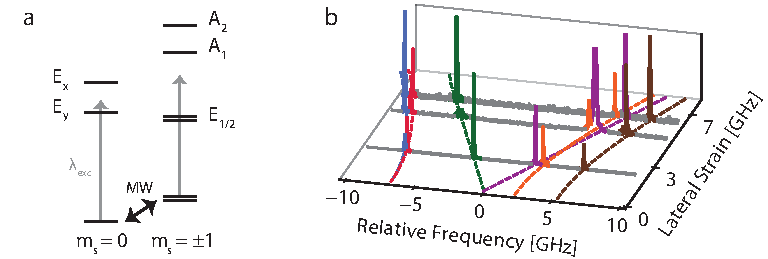
\includegraphics{laserscans}
	\caption{\label{fig:tam-fig4-laserscan} \textbf{} (a) }
\end{figure*}

\begin{figure*}
	\centering
	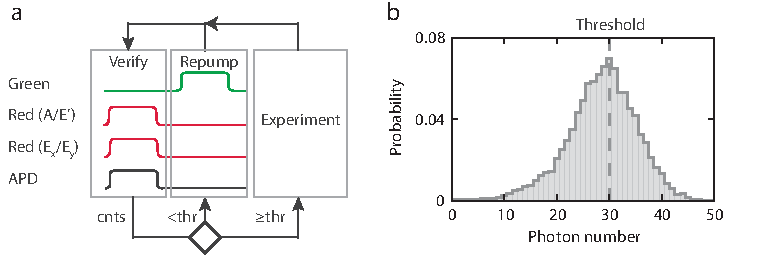
\includegraphics{CR}
	\caption{\label{fig:tam-fig4-cr} \textbf{} (a) }
\end{figure*}

\begin{figure*}
	\centering
	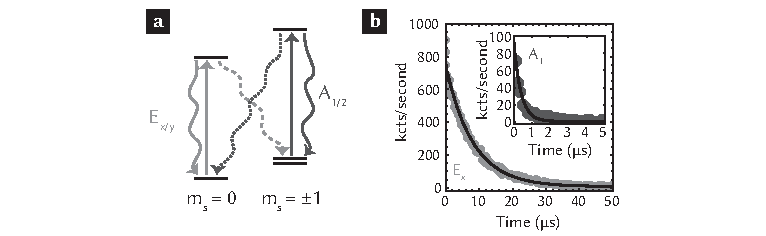
\includegraphics{figure_spinpumping-bernien}
	\caption{\label{fig:tam-fig5-SP} \textbf{} (a) }
\end{figure*}

\begin{figure*}
	\centering
	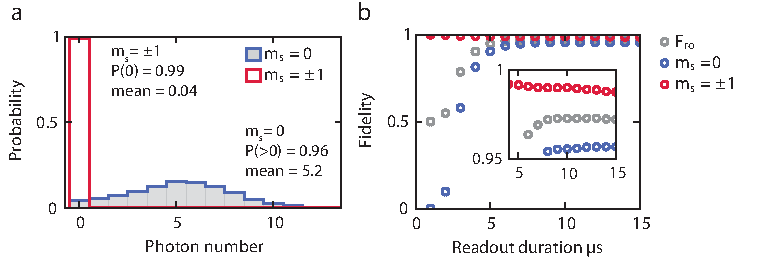
\includegraphics{ssro}
	\caption{\label{fig:tam-fig6-ssro} \textbf{} (a) }
\end{figure*}

\section{Ground state spin control and coherence}

\begin{figure*}
	\centering
	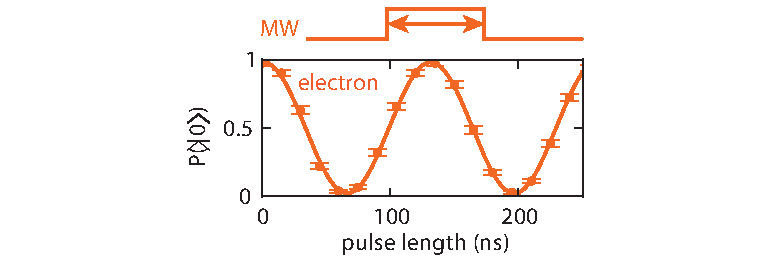
\includegraphics{electron_rabi}
	\caption{\label{fig:tam-fig7-erabi} \textbf{} (a) }
\end{figure*}

\begin{figure*}
	\centering
	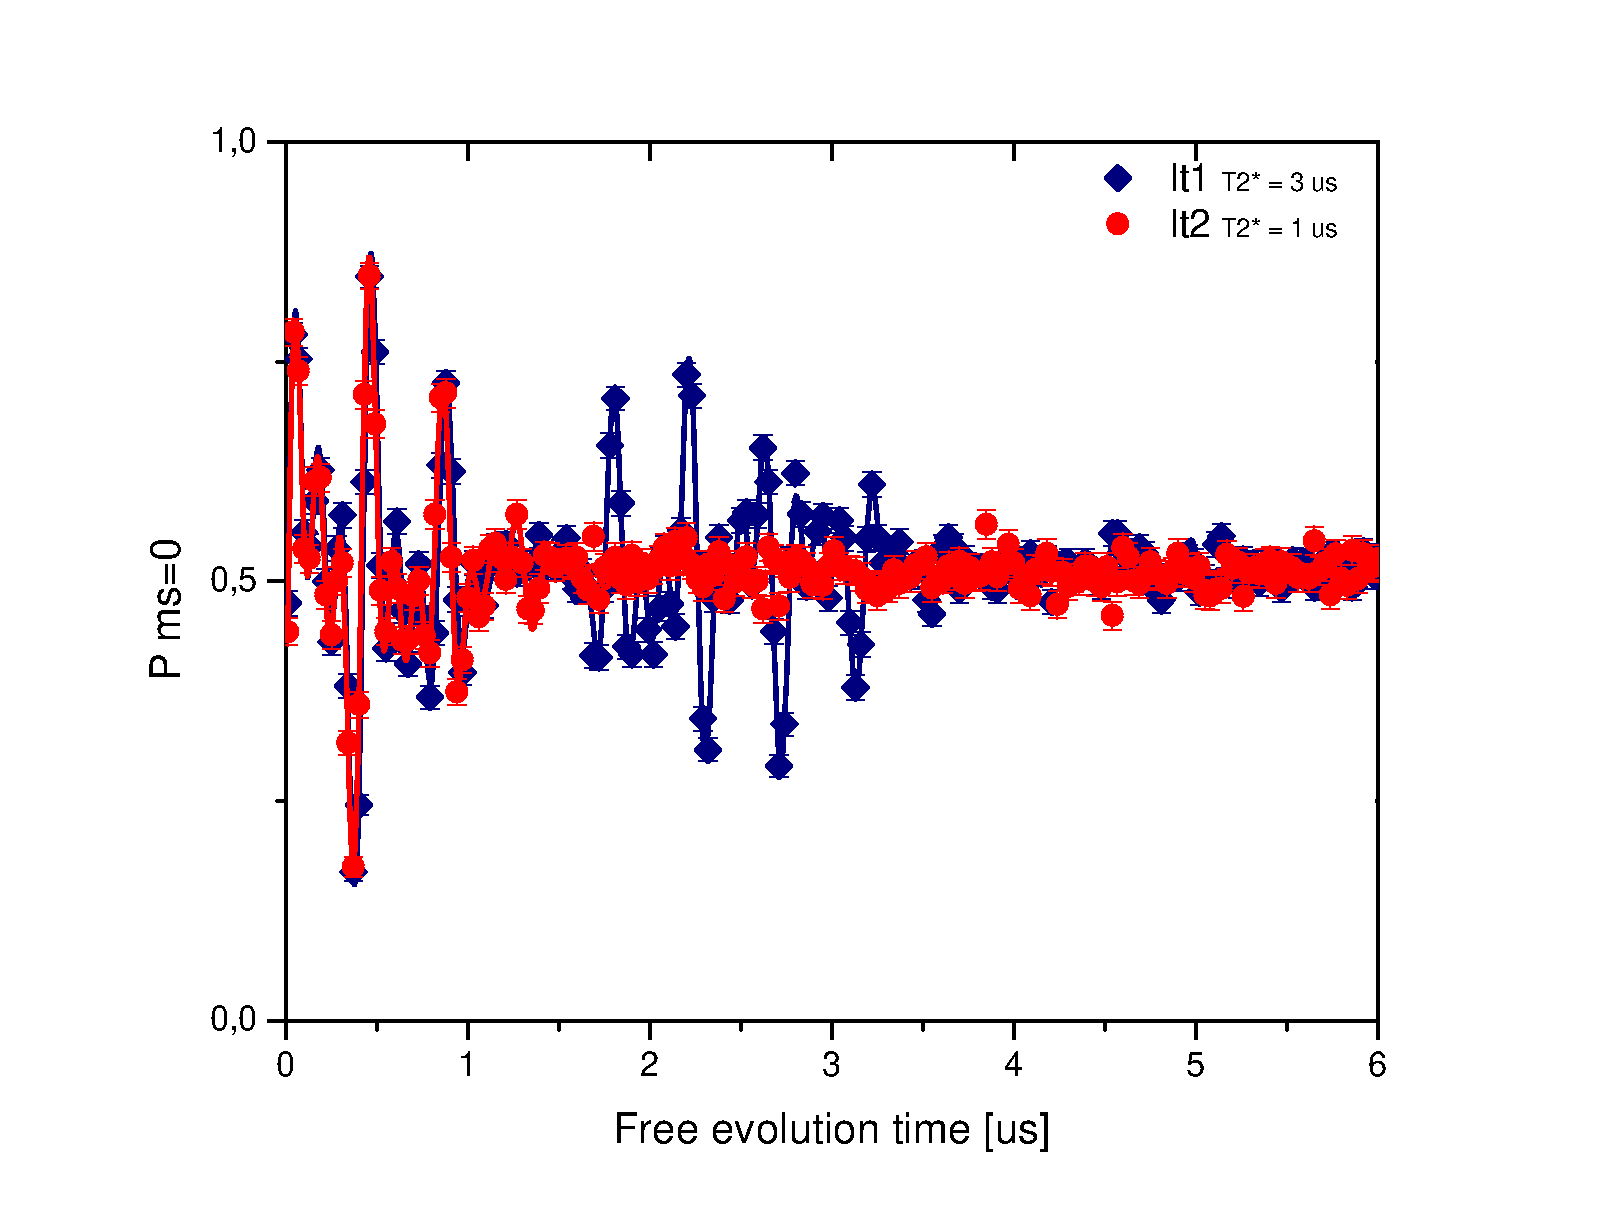
\includegraphics{ramsey-LDE}
	\caption{\label{fig:tam-fig8-eramsey} \textbf{} (a) }
\end{figure*}

\begin{figure*}
	\centering
	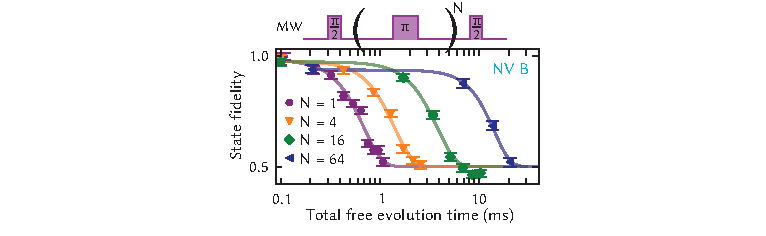
\includegraphics{DD-LDE_bernien}
	\caption{\label{fig:tam-fig9-DD} \textbf{} (a) }
\end{figure*}

\section{Coupling to nuclear spins}
\begin{figure*}
	\centering
	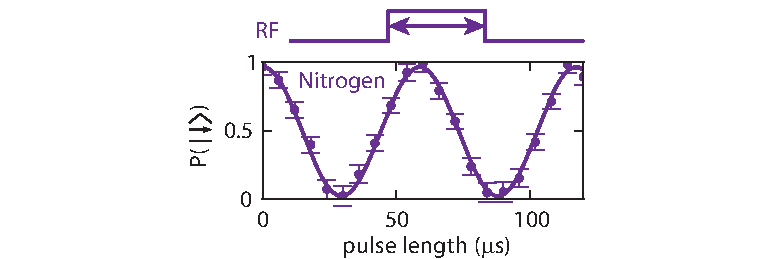
\includegraphics{nitrogen_rabi}
	\caption{\label{fig:tam-fig1-nrabi} \textbf{} (a) }
\end{figure*}
\section{Quantum measurements}


\section{Methods}



\newpage
\bibliographystyle{../thesis}
\bibliography{cdl}


